\documentclass[a4paper,14pt, unknownkeysallowed]{extreport}

\usepackage{cmap} % Улучшенный поиск русских слов в полученном pdf-файле
\usepackage[T2A]{fontenc} % Поддержка русских букв
\usepackage[utf8]{inputenc} % Кодировка utf8
\usepackage[english,russian]{babel} % Языки: русский, английский
\usepackage{enumitem}


\usepackage{threeparttable}

\usepackage[14pt]{extsizes}

\usepackage{caption}
\captionsetup{labelsep=endash}
\captionsetup[figure]{name={Рисунок}}

% \usepackage{ctable}
% \captionsetup[table]{justification=raggedleft,singlelinecheck=off}

\usepackage{amsmath}

\usepackage{geometry}
\geometry{left=30mm}
\geometry{right=10mm}
\geometry{top=20mm}
\geometry{bottom=20mm}

\usepackage{titlesec}
\titleformat{\section}
	{\normalsize\bfseries}
	{\thesection}
	{1em}{}
\titlespacing*{\chapter}{0pt}{-30pt}{8pt}
\titlespacing*{\section}{\parindent}{*4}{*4}
\titlespacing*{\subsection}{\parindent}{*4}{*4}

\usepackage{setspace}
\onehalfspacing % Полуторный интервал

\frenchspacing
\usepackage{indentfirst} % Красная строка

\usepackage{titlesec}
\titleformat{\chapter}{\LARGE\bfseries}{\thechapter}{20pt}{\LARGE\bfseries}
\titleformat{\section}{\Large\bfseries}{\thesection}{20pt}{\Large\bfseries}

\usepackage{multirow}
\usepackage{listings}
\usepackage{xcolor}

% Для листинга кода:
\lstset{%
	language=python,   					% выбор языка для подсветки	
	basicstyle=\small\sffamily,			% размер и начертание шрифта для подсветки кода
	numbers=left,						% где поставить нумерацию строк (слева\справа)
	%numberstyle=,						% размер шрифта для номеров строк
	stepnumber=1,						% размер шага между двумя номерами строк
	numbersep=5pt,						% как далеко отстоят номера строк от подсвечиваемого кода
	frame=single,						% рисовать рамку вокруг кода
	tabsize=4,							% размер табуляции по умолчанию равен 4 пробелам
	captionpos=t,						% позиция заголовка вверху [t] или внизу [b]
	breaklines=true,					
	breakatwhitespace=true,				% переносить строки только если есть пробел
	escapeinside={\#*}{*)},				% если нужно добавить комментарии в коде
	backgroundcolor=\color{white},
}


\usepackage{pgfplots}
\usetikzlibrary{datavisualization}
\usetikzlibrary{datavisualization.formats.functions}

\usepackage{graphicx}
\newcommand{\img}[3] {
	\begin{figure}[h!]
		\center{\includegraphics[height=#1]{img/#2}}
		\caption{#3}
		\label{img:#2}
	\end{figure}
}


\usepackage[justification=centering]{caption} % Настройка подписей float объектов

\usepackage[unicode,pdftex]{hyperref} % Ссылки в pdf
\hypersetup{hidelinks}

\usepackage{csvsimple}

\newcommand{\code}[1]{\texttt{#1}}





\begin{document}


\begin{titlepage}
	\newgeometry{pdftex, left=2cm, right=2cm, top=2.5cm, bottom=2.5cm}
	\fontsize{12pt}{12pt}\selectfont
	\noindent \begin{minipage}{0.15\textwidth}
		
\includegraphics[width=\linewidth]{img/b_logo.jpg}
	\end{minipage}
	\noindent\begin{minipage}{0.9\textwidth}\centering
		\textbf{Министерство науки и высшего образования Российской Федерации}\\
		\textbf{Федеральное государственное бюджетное образовательное учреждение высшего образования}\\
		\textbf{«Московский государственный технический университет имени Н. Э.~Баумана}\\
		\textbf{(национальный исследовательский университет)»}\\
		\textbf{(МГТУ им. Н. Э.~Баумана)}
	\end{minipage}
	
	\noindent\rule{18cm}{3pt}
	\newline\newline
	\noindent ФАКУЛЬТЕТ $\underline{\text{«Информатика и системы управления»~~~~~~~~~~~~~~~~~~~~~~~~~~~~~~~~~~~~~~~~~~~~~~~~~~~~~~~}}$ \newline\newline
	\noindent КАФЕДРА $\underline{\text{«Программное обеспечение ЭВМ и информационные технологии»~~~~~~~~~~~~~~~~~~~~~~~}}$\newline\newline\newline\newline\newline\newline\newline
	
	
	\begin{center}
		\noindent\begin{minipage}{1.3\textwidth}\centering
		\Large\textbf{   ~~~ Лабораторная работа №2}\newline
		\textbf{по дисциплине "Анализ Алгоритмов"}\newline\newline\newline
		\end{minipage}
	\end{center}
	
	\noindent\textbf{Тема} 			$\underline{\text{Алгоритм Копперсмита-Винограда}}$\newline\newline
	\noindent\textbf{Студент} 		$\underline{\text{Ковалец К. Э.}}$\newline\newline
	\noindent\textbf{Группа} 		$\underline{\text{ИУ7-53Б}}$\newline\newline
	\noindent\textbf{Преподаватель} $\underline{\text{Волкова Л. Л.}}$\newline
	
	\begin{center}
		\vfill
		Москва~---~\the\year
		~г.
	\end{center}
	\restoregeometry
\end{titlepage}



\renewcommand{\contentsname}{Содержание} 
\tableofcontents
\setcounter{page}{2}





\chapter*{Введение}
\addcontentsline{toc}{chapter}{Введение}

Термин «матрица» применяется во множестве разных областей: от
программирования до кинематографии. Матрица в математике – это таблица чисел, состоящая из определенного количества строк (m) и столбцов (n). Мы встречаемся с матрицами каждый день, так как любая числовая информация, занесенная в таблицу, уже в какой-то степени считается матрицей.

Алгоритм Копперсмита — Винограда — алгоритм умножения квадрат- ных матриц, предложенный Д. Копперсмитом и Ш. Виноградом. Он обладает лучшей асимптотикой среди известных алгоритмов умножения матриц. На практике алгоритм Копперсмита — Винограда не используется, так как он имеет очень большую константу пропорциональности и начина- ет выигрывать в быстродействии у других известных алгоритмов только для матриц, размер которых превышает память современных компьютеров.

Целью данной лабораторной работы является изучение и реализация алгоритмов
умножения матриц, вычисление трудоёмкости этих алгоритмов. В данной
лабораторной работе рассматривается стандартный алгоритм умножения
матриц, алгоритм Винограда и модифицированный алгоритм Винограда. 

Для достижения поставленной цели необходимо выполнить следующие задачи:

\begin{itemize}
	\item исследовать классический алгоритм умножения матриц, алгоритм Винограда и модифицированный алгоритм Винограда;
	\item сравнить существующие решения;
	\item привести схемы рассматриваемых алгоритмов (классического алгоритма умножения матриц, алгоритма Винограда и модифицированного алгоритма Винограда);
	\item описать используемые структуры данных;
	\item оценить трудоёмкость рассматриваемых алгоритмов;
	\item описать структуру разрабатываемого ПО;
	\item определить средства программной реализации;
	\item провести сравнительный анализ времени работы алгоритмов;
	\item провести модульное тестирование;
	\item описать и обосновать полученные результаты в отчете о выполненной лабораторной работе, выполненном как расчётно-пояснительная
	записка к работе.
\end{itemize}





\chapter{Аналитическая часть}
В этом разделе будут представлены описания алгоритмов стандартного умножения матриц и алгоритм Копперсмита-Винограда. [1]

\section{Стандартный алгоритм}

Пусть даны две прямоугольные матрицы
\begin{equation}
	A_{lm} = \begin{pmatrix}
		a_{11} & a_{12} & \ldots & a_{1m}\\
		a_{21} & a_{22} & \ldots & a_{2m}\\
		\vdots & \vdots & \ddots & \vdots\\
		a_{l1} & a_{l2} & \ldots & a_{lm}
	\end{pmatrix},
	\quad
	B_{mn} = \begin{pmatrix}
		b_{11} & b_{12} & \ldots & b_{1n}\\
		b_{21} & b_{22} & \ldots & b_{2n}\\
		\vdots & \vdots & \ddots & \vdots\\
		b_{m1} & b_{m2} & \ldots & b_{mn}
	\end{pmatrix},
\end{equation}

тогда матрица $C$
\begin{equation}
	C_{ln} = \begin{pmatrix}
		c_{11} & c_{12} & \ldots & c_{1n}\\
		c_{21} & c_{22} & \ldots & c_{2n}\\
		\vdots & \vdots & \ddots & \vdots\\
		c_{l1} & c_{l2} & \ldots & c_{ln}
	\end{pmatrix},
\end{equation}

где
\begin{equation}
	\label{eq:M}
	c_{ij} =
	\sum_{r=1}^{m} a_{ir}b_{rj} \quad (i=\overline{1,l}; j=\overline{1,n})
\end{equation}

будет называться произведением матриц $A$ и $B$. Стандартный алгоритм реализует данную формулу.

\section{Алгоритм Копперсмита-Винограда}

\textbf{Алгоритм Копперсмита-Винограда} — алгоритм умножения квадратных матриц, предложенный в 1987 году Д. Копперсмитом и Ш. Виноградом.
В исходной версии асимптотическая сложность алгоритма составляла $O(n^{2,3755})$, где  $n$ — размер стороны матрицы.
Алгоритм Копперсмита — Винограда, с учетом серии улучшений и доработок в последующие годы, обладает лучшей асимптотикой среди известных алгоритмов умножения матриц.


Рассмотрим два вектора $V = (v_1, v_2, v_3, v_4)$ и $W = (w_1, w_2, w_3, w_4)$.
Их скалярное произведение равно: $V \cdot W = v_1w_1 + v_2w_2 + v_3w_3 + v_4w_4$, что эквивалентно (\ref{for:new}):
\begin{equation}
	\label{for:new}
	V \cdot W = (v_1 + w_2)(v_2 + w_1) + (v_3 + w_4)(v_4 + w_3) - v_1v_2 - v_3v_4 - w_1w_2 - w_3w_4.
\end{equation}

Несмотря на то, что второе выражение требует вычисления большего количества операций, чем стандартный алгоритм: вместо четырех умножений - шесть, а вместо трех сложений - десять, выражение в правой части последнего равенства допускает предварительную обработку: его части можно вычислить заранее и запомнить для каждой строки первой матрицы и для каждого столбца второй, что позволит для каждого элемента выполнять лишь два умножения и пять сложений, складывая затем только лишь с 2 предварительно посчитанными суммами соседних элементов текущих строк и столбцов.
Из-за того, что операция сложения быстрее операции умножения в ЭВМ, на практике алгоритм должен работать быстрее стандартного.

В случае нечетного значений размера изначальной матрицы ($n$), следует произвести еще одну операцию - добавление произведения последних элементов соответствующих строк и столбцов.

\section*{Вывод}
Были рассмотрены алгоритмы классического умножения матриц и алгоритм Винограда, основное отличие которого от классического алгоритма — наличие предварительной обработки, а также количество операций умножения.

На вход алгоритмам будут поступать две матрицы, кол-во столбцов первой матрицы должно совпадать с кол-вом строк второй матрицы. При попытке ввести пустые матрицы будет выдано сообщение об ошибке. Реализуемое ПО будет давать возможность выбрать алгоритм и вывести для него результат вычисления, а также возможность произвести сравнение алгоритмов по затраченному времени.



\chapter{Конструкторская часть}
В данном разделе будут приведены схемы алгоритмов умножения матриц, приведено описание используемых типов данных, оценка трудоёмкости алгоритмов, а также описана структура ПО.

\section{Схемы алгоритмов}

На вход алгоритмов падаются матрицы $matr1$ и matr2, на выходе получаем результат перемножения двух матриц, записанный в $res\_matr$.

На рис. \ref{fig:сlassic} - \ref{fig:optimized_winograd2} приведены схемы стандартного алгоритма умножения матриц, алгоритма Винограда и оптимизированного алгоритма Винограда.

\clearpage

\begin{figure}[h]
	\centering
	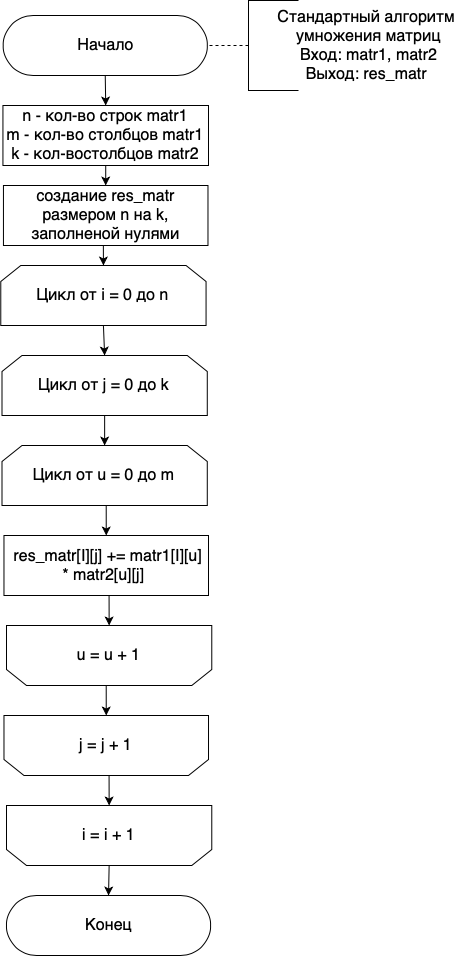
\includegraphics[scale=0.7]{img/classical_alg_scheme.png}
	\caption{Схема стандартного алгоритма умножения матриц}
	\label{fig:сlassic}
\end{figure}

\clearpage

\begin{figure}[h]
	\centering
	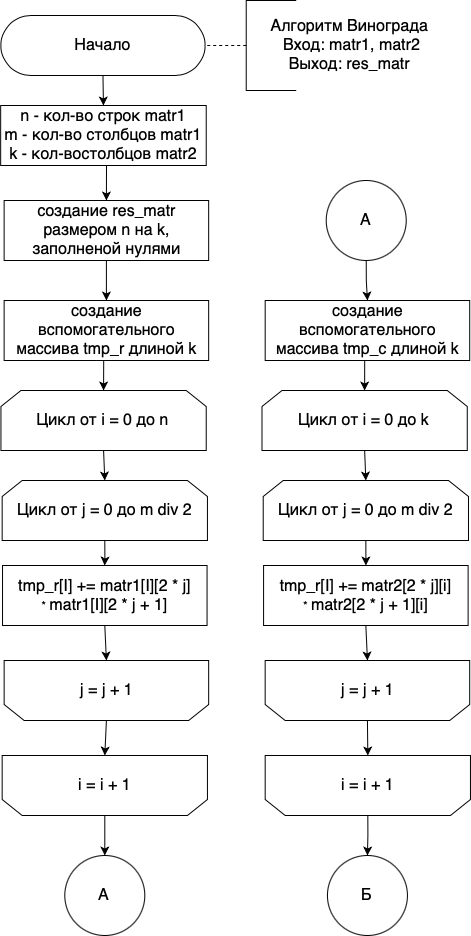
\includegraphics[scale=0.7]{img/winograd_alg_scheme1.png}
	\caption{Схема умножения матриц алгоритмом Винограда}
	\label{fig:winograd1}
\end{figure}
 
\clearpage

\begin{figure}[h]
	\centering
	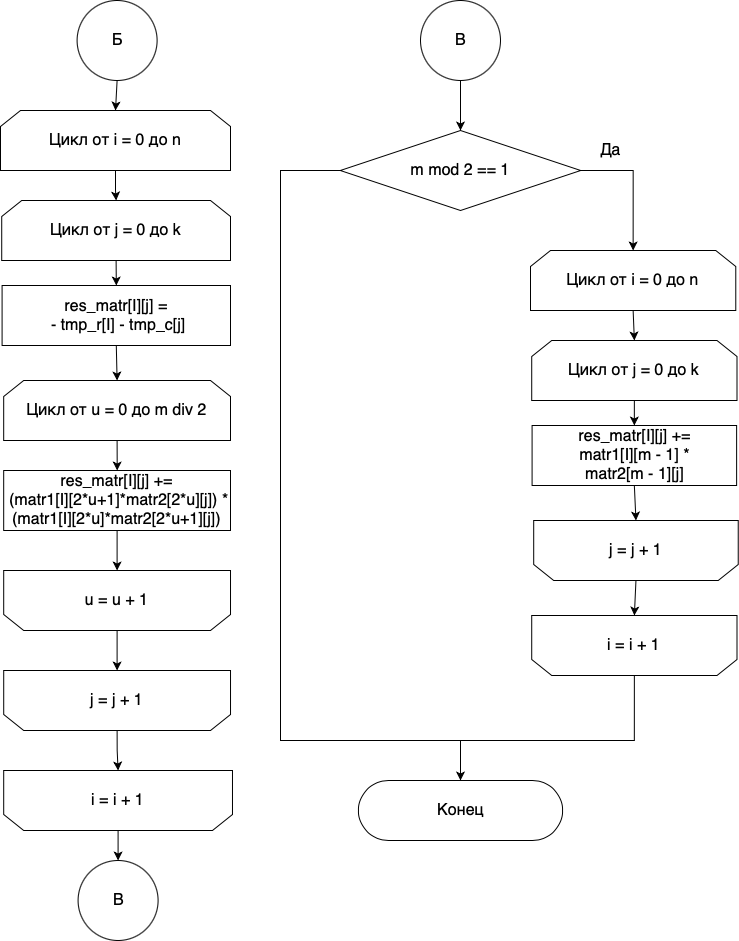
\includegraphics[scale=0.67]{img/winograd_alg_scheme2.png}
	\caption{Схема умножения матриц алгоритмом Винограда (продолжение)}
	\label{fig:winograd2}
\end{figure}

\clearpage

\begin{figure}[h]
	\centering
	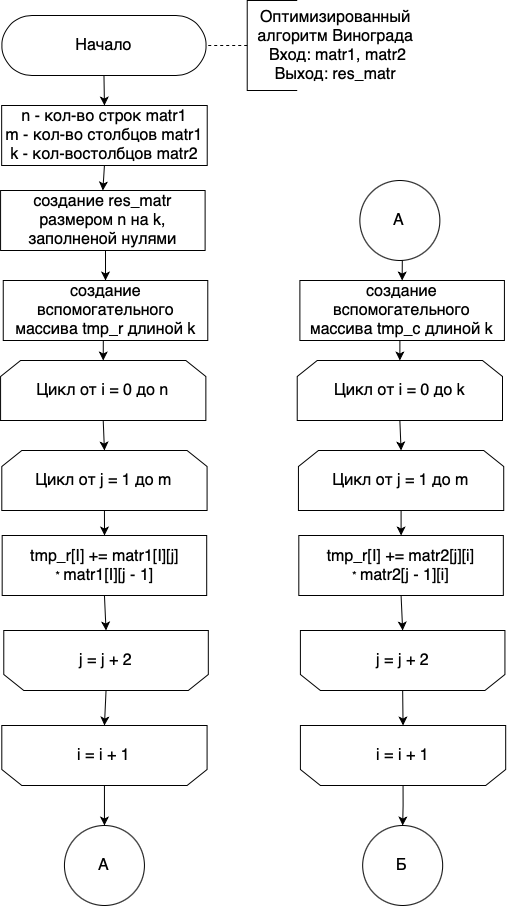
\includegraphics[scale=0.7]{img/optimized_winograd_alg_scheme1.png}
	\caption{Схема умножения матриц оптимизированным алгоритмом Винограда}
	\label{fig:optimized_winograd1}
\end{figure}

\clearpage

\begin{figure}[h]
	\centering
	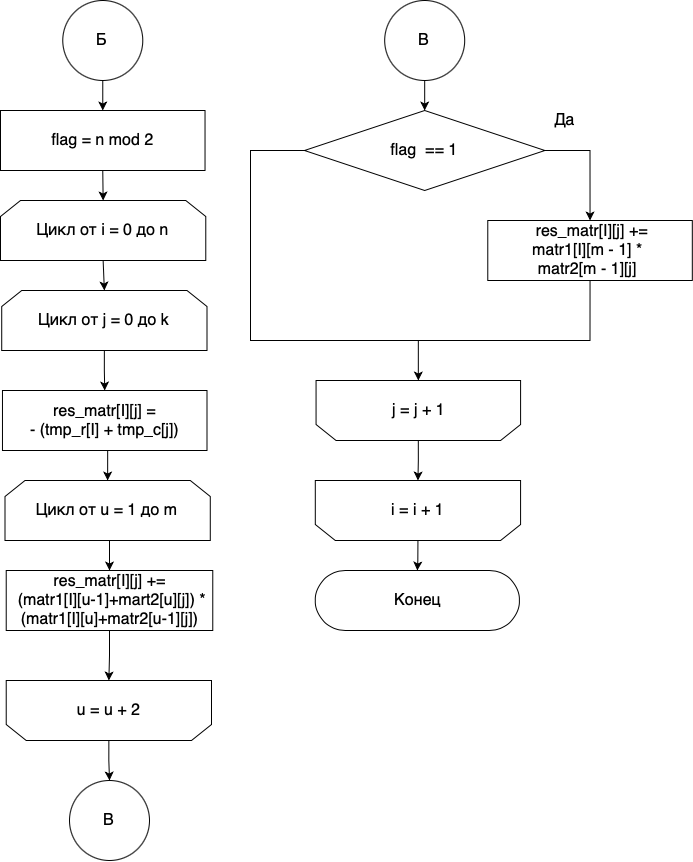
\includegraphics[scale=0.7]{img/optimized_winograd_alg_scheme2.png}
	\caption{Схема умножения матриц оптимизированным алгоритмом Винограда (продолжение)}
	\label{fig:optimized_winograd2}
\end{figure}

\clearpage

\section{Модель вычислений}

Для последующего вычисления трудоемкости необходимо ввести модель вычислений:
\begin{enumerate}
	\item операции из списка (\ref{for:opers}) имеют трудоемкость 1;
	\begin{equation}
		\label{for:opers}
		+, -, *, /, \%, ==, !=, <, >, <=, >=, [], ++, {-}-
	\end{equation}
	\item трудоемкость оператора выбора \code{if условие then A else B} рассчитывается, как (\ref{for:if});
	\begin{equation}
		\label{for:if}
		f_{if} = f_{\text{условия}} +
		\begin{cases}
			f_A, & \text{если условие выполняется,}\\
			f_B, & \text{иначе.}
		\end{cases}
	\end{equation}
	\item трудоемкость цикла рассчитывается, как (\ref{for:for});
	\begin{equation}
		\label{for:for}
		f_{for} = f_{\text{инициализации}} + f_{\text{сравнения}} + N(f_{\text{тела}} + f_{\text{инкремента}} + f_{\text{сравнения}})
	\end{equation}
	\item трудоемкость вызова функции равна 0.
\end{enumerate}


\section{Трудоемкость алгоритмов}

В следующих частях будут расчитаны трудоемкости алгоритмов умножения матриц.

\subsection{Стандартный алгоритм умножения матриц}

Во всех последующих алгоритмах не будем учитывать инициализацию матрицы, в которую записывается результат, потому что данное действие есть во всех алгоритмах и при этом не является самым трудоёмким.

Трудоёмкость стандартного алгоритма умножения матриц состоит из:
\begin{itemize}
	\item внешнего цикла по $i \in [1..M]$, трудоёмкость которого: $f = 2 + M \cdot (2 + f_{body})$;
	\item цикла по $j \in [1..N]$, трудоёмкость которого: $f = 2 + N \cdot (2 + f_{body})$;
	\item цикла по $k \in [1..K]$, трудоёмкость которого: $f = 2 + 10K$;
\end{itemize}

Учитывая, что трудоёмкость стандартного алгоритма равна трудоёмкости внешнего цикла, можно вычислить ее, подставив циклы тела (\ref{for:standard}):
\begin{equation}
	\label{for:standard}
	f_{standard} = 2 + M \cdot (4 + N \cdot (4 + 10K)) = 2 + 4M + 4MN + 10MNK \approx 10MNK
\end{equation}

\subsection{Алгоритм Копперсмита — Винограда}

Трудоёмкость алгоритма Копперсмита — Винограда состоит из:
\begin{itemize}
	\item создания и инициализации массивов MH и MV, трудоёмкость которого (\ref{for:init}):
	\begin{equation}
		\label{for:init}
		f_{init} = M + N;
	\end{equation}
	
	\item заполнения массива MH, трудоёмкость которого (\ref{for:MH}):
	\begin{equation}
		\label{for:MH}
		f_{MH} = 2 + K (2 + \frac{M}{2} \cdot 11);
	\end{equation}
	
	\item заполнения массива MV, трудоёмкость которого (\ref{for:MV}):
	\begin{equation}
		\label{for:MV}
		f_{MV} = 2 + K (2 + \frac{N}{2} \cdot 11);
	\end{equation}
	
	\item цикла заполнения для чётных размеров, трудоёмкость которого (\ref{for:cycle}):
	\begin{equation}
		\label{for:cycle}
		f_{cycle} = 2 + M \cdot (4 + N \cdot (11 + \frac{K}{2} \cdot 23));
	\end{equation}
	
	\item цикла, для дополнения умножения суммой последних нечётных строки и столбца, если общий размер нечётный, трудоемкость которого (\ref{for:last}):
	\begin{equation}
		\label{for:last}
		f_{last} = \begin{cases}
			2, & \text{чётная,}\\
			4 + M \cdot (4 + 14N), & \text{иначе.}
		\end{cases}
	\end{equation}
\end{itemize}

Итого, для худшего случая (нечётный общий размер матриц) имеем (\ref{for:bad}):
\begin{equation}
	\label{for:bad}
	f =  f_{MH} + f_{MV} + f_{cycle} + f_{last}\approx 11.5 \cdot MNK
\end{equation}

Для лучшего случая (чётный общий размер матриц) имеем (\ref{for:good}):
\begin{equation}
	\label{for:good}
f =  f_{MH} + f_{MV} + f_{cycle} + f_{last} \approx 11.5 \cdot MNK
\end{equation}


\subsection{Оптимизированный алгоритм Копперсмита — Винограда}

Оптимизированный алгоритм Винограда представляет собой обычный алгоритм Винограда, за исключением следующих оптимизаций:
\begin{itemize}
	\item вычисление происходит заранее;
	\item используется битовый сдвиг, вместо деления на 2;
	\item последний цикл для нечётных элементов включён в основной цикл,
	используя дополнительные операции в случае нечётности N.
\end{itemize}


Трудоёмкость улучшенного алгоритма Копперсмита — Винограда состоит из:
\begin{itemize}
	\item создания и инициализации массивов MH и MV, трудоёмкость которого (\ref{for:impr_init}):
	\begin{equation}
		\label{for:impr_init}
		f_{init} = M + N;
	\end{equation}
	
	\item заполнения массива MH, трудоёмкость которого (\ref{for:impr_MH}):
	\begin{equation}
		\label{for:impr_MH}
		f_{MH} =  2 + K (2 + \frac{M}{2} \cdot 8);
	\end{equation}
	
	\item заполнения массива MV, трудоёмкость которого (\ref{for:impr_MV}):
	\begin{equation}
		\label{for:impr_MV}
		f_{MV} =  2 + K (2 + \frac{M}{2} \cdot 8);
	\end{equation}
	
	\item цикла заполнения для чётных размеров, трудоёмкость которого (\ref{for:impr_cycle}):
	\begin{equation}
		\label{for:impr_cycle}
		f_{cycle} =2 + M \cdot (4 + N \cdot (11 + \frac{K}{2} \cdot 18));
	\end{equation}
	
	\item условие, для дополнения умножения суммой последних нечётных строки и столбца, если общий размер нечётный, трудоемкость которого (\ref{for:impr_last}):
	\begin{equation}
		\label{for:impr_last}
		f_{last} = 
		\begin{cases}
			1, & \text{чётная,}\\
			4 + M \cdot (4 + 10N), & \text{иначе.}
		\end{cases}
	\end{equation}
\end{itemize}

Итого, для худшего случая (нечётный общий размер матриц) имеем (\ref{for:bad_impr}):
\begin{equation}
	\label{for:bad_impr}
	f = f_{MH} + f_{MV} + f_{cycle} + f_{last} \approx 9MNK
\end{equation}

Для лучшего случая (чётный общий размер матриц) имеем (\ref{for:good_impr}):
\begin{equation}
	\label{for:good_impr}
	f = f_{MH} + f_{MV} + f_{cycle} + f_{last} \approx 9MNK
\end{equation}

\section{Классы эквивалентности}

Выделенные классы эквивалентности для тестирования:

\begin{itemize}
	\item ввод пустых матриц;
	\item одна из матриц - пустая;
	\item кол-во столбцов первой матрицы не равно кол-ву строк второй матрицы;
	\item перемножение квадратных матриц;
	\item перемножение матриц разных размеров (кол-во столбцов первой матрицы равно кол-ву строк второй матрицы).
\end{itemize}

\clearpage

\section{Описание используемых типов данных}

При реализации алгоритмов будут использованы следующие структуры данных:

\begin{itemize}
	\item кол-во строк в матрице - целое число типа $int$;
	\item кол-во столбцов в матрице - целое число типа $int$;
	\item матрица - двумерный массив типа $int$.
\end{itemize}

\section{Структура ПО}

ПО будет состоять из следующих модулей:

\begin{itemize}
	\item $main.py$ - файл, содержащий функцию $main$;
    \item $matrix\_mult.py$ - файл, содержащий код всех алгоритмов умножения матриц и функций, отвечающих за умножение;
    \item $compare\_time.py$ - файл, в котором содержатся функции для замера времени работы алгоритмов;
    \item $in\_out\_matrix.py$ - файл, в котором содержатся функции ввода-вывода матриц;
    \item $color.py$ - файл, который содержит переменные типа $string$ для цветного вывода результата работы программы в консоль.
\end{itemize}

\section{Вывод}

В данном разделе на основе теоретических данных были построены схемы требуемых алгоритмов умножения матриц, выбраны используемые типы данных, выделены классы эквивалентности для тестирования, а также была проведена оценка трудоёмкости алгоритмов и описана структура ПО.

\clearpage





\chapter{Технологическая часть}

В данном разделе будут приведены требования к программному обеспечению, средства реализации, листинги кода, а также функциональные тесты.

\section{Требования к программному обеспечению}

\begin{itemize}
    \item входные данные - две матрицы $matr1$ и $matr2$, кол-во столбцов матрицы $matr1$ должно совпадать с кол-вом строк матрицы $matr2$;
    \item выходные данные - резульат умножения входных матриц ($res\_matr$).
\end{itemize}

\section{Средства реализации}
В данной работе для реализации был выбран язык программирования $Python$ [2]. Выбор обсуловлен наличием опыта работы с ним. Время работы было замерено с помощью функции \textit{process\_time} из библиотеки $time$ [3].

\clearpage

\section{Листинги кода}

В листингах \ref{lst:classical_alg} - \ref{lst:optimized_winograd_alg} представлены реализации алгоритмов умножения матриц.

\begin{center}
\captionsetup{justification=raggedright,singlelinecheck=off}
\begin{lstlisting}[label=lst:classical_alg,caption=Функция стандартного алгоритма умножения матриц]
def classical_alg(matr1, matr2):

    n = len(matr1)
    m = len(matr1[0])
    k = len(matr2[0])

    res_matr = [[0] * k for _ in range(n)]

    for i in range(n):
        for j in range(k):
            for u in range(m):
                res_matr[i][j] += matr1[i][u] * matr2[u][j]

    return res_matr
\end{lstlisting}
\end{center}

\clearpage

\begin{center}
\captionsetup{justification=raggedright,singlelinecheck=off}
\begin{lstlisting}[label=lst:winograd_alg,caption=Функция умножения матриц алгоритмом Винограда]
def winograd_alg(matr1, matr2):

    n = len(matr1)
    m = len(matr1[0])
    k = len(matr2[0])

    res_matr = [[0] * k for _ in range(n)]

    tmp_r = [0] * n
    for i in range(n):
        for j in range(0, m // 2, 1):
            tmp_r[i] += matr1[i][2 * j] * matr1[i][2 * j + 1]

    tpm_c = [0] * k
    for i in range(k):
        for j in range(0, m // 2, 1):
            tpm_c[i] += matr2[2 * j][i] * matr2[2 * j + 1][i]

    for i in range(n):
        for j in range(k):
            res_matr[i][j] = -tmp_r[i] - tpm_c[j]

            for u in range(0, m // 2, 1):
                res_matr[i][j] += (matr1[i][2 * u + 1] + matr2[2 * u    ][j]) * \
                                  (matr1[i][2 * u    ] + matr2[2 * u + 1][j])

    if m % 2 == 1:
        for i in range(n):
            for j in range(k):
                res_matr[i][j] += matr1[i][m - 1] * matr2[m - 1][j]

    return res_matr
\end{lstlisting}
\end{center}

\clearpage

\begin{center}
\captionsetup{justification=raggedright,singlelinecheck=off}
\begin{lstlisting}[label=lst:optimized_winograd_alg,caption=Функция умножения матриц оптимизированным алгоритмом Винограда]
def optimized_winograd_alg(matr1, matr2):

    n = len(matr1)
    m = len(matr1[0])
    k = len(matr2[0])

    res_matr = [[0] * k for _ in range(n)]

    tmp_r = [0] * n
    for i in range(n):
        for j in range(1, m, 2):
            tmp_r[i] += matr1[i][j] * matr1[i][j - 1]

    tpm_c = [0] * k
    for i in range(k):
        for j in range(1, m, 2):
            tpm_c[i] += matr2[j][i] * matr2[j - 1][i]

    flag = n % 2
    for i in range(n):
        for j in range(k):
            res_matr[i][j] = -(tmp_r[i] + tpm_c[j])

            for u in range(1, m, 2):
                res_matr[i][j] += (matr1[i][u - 1] + matr2[u    ][j]) * \
                                  (matr1[i][u    ] + matr2[u - 1][j])
            if flag:
                res_matr[i][j] += matr1[i][m - 1] * matr2[m - 1][j]

    return res_matr
\end{lstlisting}
\end{center}

\clearpage

\section{Функциональные тесты}

В таблице \ref{tbl:functional_test} приведены функциональные тесты для алгоритмов умнжения матриц (стандартного алгоритма, алгоритма Винограда и оптимизированного алгоритма Винограда). Все тесты пройдены успешно.

\begin{table}[h]
	\begin{center}
	\begin{threeparttable}
		\captionsetup{justification=raggedright,singlelinecheck=off}
		\caption{\label{tbl:functional_test} Функциональные тесты}
		\begin{tabular}{|c|c|c|}
			\hline
			1-ая матрица & 2-ая матрица & Ожидаемый результат 
			\\ \hline
			$\begin{pmatrix}
				\\
			 \end{pmatrix}$ &
			 $\begin{pmatrix}
				\\
			 \end{pmatrix}$ &
			Сообщение об ошибке

			\\ \hline
			$\begin{pmatrix}
				\\
			 \end{pmatrix}$ &
			$\begin{pmatrix}
				1 & 1\\
				1 & 1
			 \end{pmatrix}$ &
			Сообщение об ошибке

			\\ \hline
			$\begin{pmatrix}
				0 & 1
			 \end{pmatrix}$ &
			$\begin{pmatrix}
				0 & 1
			\end{pmatrix}$ &
			Сообщение об ошибке 
			
			\\ \hline
			$\begin{pmatrix}
				5
			 \end{pmatrix}$ &
			$\begin{pmatrix}
				5
			\end{pmatrix}$ &
			$\begin{pmatrix}
				25
			\end{pmatrix}$

			\\ \hline
			$\begin{pmatrix}
				1 & 2 & 3\\
				4 & 5 & 6\\
				7 & 8 & 9
			\end{pmatrix}$ &
			$\begin{pmatrix}
				1 & 2 & 3\\
				4 & 5 & 6\\
				7 & 8 & 9
			\end{pmatrix}$ &
			$\begin{pmatrix}
				30 & 36 & 42\\
				66 & 81 & 96\\
				102 & 126 & 150
			\end{pmatrix}$ 
			                 
			\\ \hline
			$\begin{pmatrix}
				1 & 2 & 3
			\end{pmatrix}$ &
			$\begin{pmatrix}
				1\\
				2\\
				3
			\end{pmatrix}$ &
			$\begin{pmatrix}
				14
			\end{pmatrix}$ 

			\\ \hline
			$\begin{pmatrix}
				1 & 2 & 3 \\
				4 & 5 & 6 \\
				7 & 8 & 9
			\end{pmatrix}$ &
			$\begin{pmatrix}
				1 & 4\\
				2 & 5\\
				3 & 6
			\end{pmatrix}$ &
			$\begin{pmatrix}
				14 & 32 \\
				32 & 77 \\
				50 & 122
			\end{pmatrix}$                  
			\\ \hline
		\end{tabular}
	\end{threeparttable}
	\end{center}
\end{table}

\section{Вывод}

В данном разделе были разработаны алгоритмы умножения матриц (стандартный, Винограда и оптимизированный Винограда), проведено тестирование, описаны средства реализации и требования к ПО.





\chapter{Исследовательская часть}

\section{Технические характеристики}

Технические характеристики устройства, на котором выполнялось тестирование представлены далее.

\begin{itemize}
    \item Операционная система: macOS 11.5.2. [4]
    \item Память: 8 GiB.
    \item Процессор: 2,3 GHz 4‑ядерный процессор Intel Core i5. [5]
\end{itemize}

При тестировании ноутбук был включен в сеть электропитания. Во время тестирования ноутбук был нагружен только встроенными приложениями окружения, а также системой тестирования.

\section{Демонстрация работы программы}

\img{180mm}{example}{Пример работы программы}
\clearpage

\section{Время выполнения алгоритмов}

Результаты замеров времени работы алгоритмов умножения матриц (стандартного, Винограда и оптимизированного Винограда) приведены на рисунках 4.2 - 4.5. Замеры времени проводились на квадратных матрицах чётного и нечётного размеров (в секундах) и усреднялись для каждого набора одинаковых экспериментов.

\img{40mm}{time_measurements_table1}{Cравнение алгоритмов по времени при чётных размерах квадратных матриц в таблице}
\img{114mm}{time_measurements1}{Сравнение алгоритмов по времени при чётных размерах квадратных матриц}
\clearpage

\img{40mm}{time_measurements_table2}{Cравнение алгоритмов по времени при нечётных размерах квадратных матриц в таблице}
\img{114mm}{time_measurements2}{Сравнение алгоритмов по времени при нечётных размерах квадратных матриц}
\clearpage

\section{Вывод}

В этом разделе были указаны технические характеристики машины, на которой происходило сравнение времени работы алгоритмов умножения матриц, а также приведены результаты исследования.

Сравнения проводились на квадратных матрицах чётного и нечётного размеров. В обоих случаях алгоритм Винограда показал наихудший результат. На матрицах размером 200x200 он работал на 24.8\% времени дольше, чем оптимизированный алгоритм Винограда и на 23.8\% дольше стандартного алгоритма. На матрицах 199x199 на 26.3\% и 25.3\% соответственно. На матрицах большего размера разница оставалась похожей (28.5\% и 27.8\% на матрицах 350x350 и 27.2\% и 28.5\% на матрицах 349x349). Стандартный алгоритм умножения матриц и оптимизированный алгоритм Винограда показали схожие результаты при чётных и нечётных размерах матриц. На матрицах размером 350x350 оптимизированный алгоритм Винограда работает на 0.6\% быстрее стандартного алгоритма, а на матрицах 349x349 на 1.0\% медленее его. 
 

\chapter*{Заключение}
\addcontentsline{toc}{chapter}{Заключение}

Было экспериментально подтверждено различие во временной эффективности стандартного алгоритма умножения матриц, алгоритма Винограда и оптимизированного алгоритма Винограда.

В результате исследований можно сделать вывод о том, что алгоритм Винограда неэффективен по времени на матрицах малого размера (350x350 и меньше).

\vspace{5mm}

В ходе выполнения данной лабораторной работы были решены следующие задачи:
\begin{itemize}
	\item изучены стандартный алгоритма умножения матриц, алгоритм Винограда и оптимизированный алгоритм Винограда;
	\item реализованы указанные алгоритмы;
	\item проведен сравнительный анализ трудоёмкости алгоритмов на основе теоретических расчетов и выбранной модели вычислений;
	\item экспериментально подтверждено различие во временнoй эффективности алгоритмов умножения матриц при помощи разработанного программного обеспечения на материале замеров процессорного времени;
	\item описаны и обоснованы полученные результаты в отчете о выполненной лабораторной работе, выполненного как расчётно-пояснительная записка к работе.
\end{itemize}

Поставленная цель была достигнута.


\begin{thebibliography}{5}
	\bibitem{bib1}
	Умножение матриц [Электронный ресурс],
	howpublished="Режим доступа: \url{http://algolib.narod.ru/Math/Matrix.html} (дата обращения: 18.10.2021).
	\bibitem{bib2}
	Welcome to Python [Электронный ресурс]. Режим доступа: \url{https://www.python.org} (дата обращения: 18.10.2021).
	\bibitem{bib3}
	time — Time access and conversions [Электронный ресурс]. Режим доступа: \url{https://docs.python.org/3/library/time.html#functions} (дата обращения: 18.10.2021).
	\bibitem{bib4}
	macOS Monterey - Apple(RU) [Электронный ресурс]. Режим доступа: \url{https://www.apple.com/ru/macos/monterey/} (дата обращения: 18.10.2021).
	\bibitem{bib5}
	Intel [Электронный ресурс]. Режим доступа: \url{https://www.intel.ru/content/www/ru/ru/products/details/processors/core/i5.html} (дата обращения: 18.10.2021).
\end{thebibliography}

\addcontentsline{toc}{chapter}{Список литература}

\end{document}
